%
% section 5.1.4
%
\setcounter{subsection}{3}
\subsection{Τεχνολογίες Ψηφιακής Συνδρομητικής Γραμμής (xDSL)}

Το ακρωνύμιο DSL προέρχεται από τις λέξεις \emph{Digital Subscriber Line} και αποτελεί μια τεχνολογία που μετατρέπει την απλή τηλεφωνική γραμμή σε ένα δίαυλο μεταφοράς ψηφιακών δεδομένων υψηλής ταχύτητας και μεγάλου εύρους ζώνης με τη χρήση ειδικών modems που τοποθετούνται στα άκρα της γραμμής. Τα modems αυτά χρησιμοποιούν αισθητά μεγαλύτερες συχνότητες από αυτές που χρησιμοποιούνται για τη φωνή (όπως είδαμε στην προηγούμενη ενότητα  η τηλεφωνική γραμμή μπορεί να τις μεταφέρει) και για το λόγο αυτό ονομάζονται και \emph{broadband modems}. Κατά τα άλλα τα broadband modems  λειτουργούν με τον ίδιο τρόπο λειτουργίας των κλασικών modems, μετατρέπουν δηλ. τη ροή ψηφιακού σήματος  σε αναλογικό σήμα υψηλού ρυθμού (υψηλής συχνότητας). Η γραμμή μπορεί να μεταφέρει ταυτόχρονα χωρίς πρόβλημα τη φωνή και τα δεδομένα καθώς οι συχνότητες που χρησιμοποιούνται για τις δυο μεταδόσεις απέχουν αρκετά μεταξύ τους και μπορούν να ξεχωρίσουν εύκολα (αυτή τη δουλειά κάνει το φίλτρο ή ο διαχωριστής (splitter) που βάζουμε στην τηλεφωνική γραμμή).

Στη μετάδοση δεδομένων DSL χρησιμοποιούνται διάφορες τεχνολογίες διαμόρφωσης οι οποίες επιτυγχάνουν διαφορετικές ταχύτητες. Το διαθέσιμο εύρος ζώνης της γραμμής χωρίζεται σε τρία κανάλια:

\begin{itemize}
\item Ένα για τη μετάδοση φωνής
\item Ένα για τη μετάδοση δεδομένων προς τα πάνω (από το συνδρομητή προς τον παροχέα), γνωστό ως \emph{upstream}
\item Ένα για τη μετάδοση δεδομένων προς τα κάτω (από τον παροχέα προς το συνδρομητή), γνωστό ως \emph{downstream}
\end{itemize}

Οι επιδόσεις που επιτυγχάνονται διαφέρουν ανάλογα με το modem που θα συνδέσουμε. Με την τεχνολογία DSL επιτυγχάνονται ταχύτητες μέχρι 52 Mbps down\-stream και 12 Mbps upstream ενώ  μεταδίδεται ταυτόχρονα και το αναλογικό σήμα φωνής.

\begin{figure}[!ht]
  \centering
  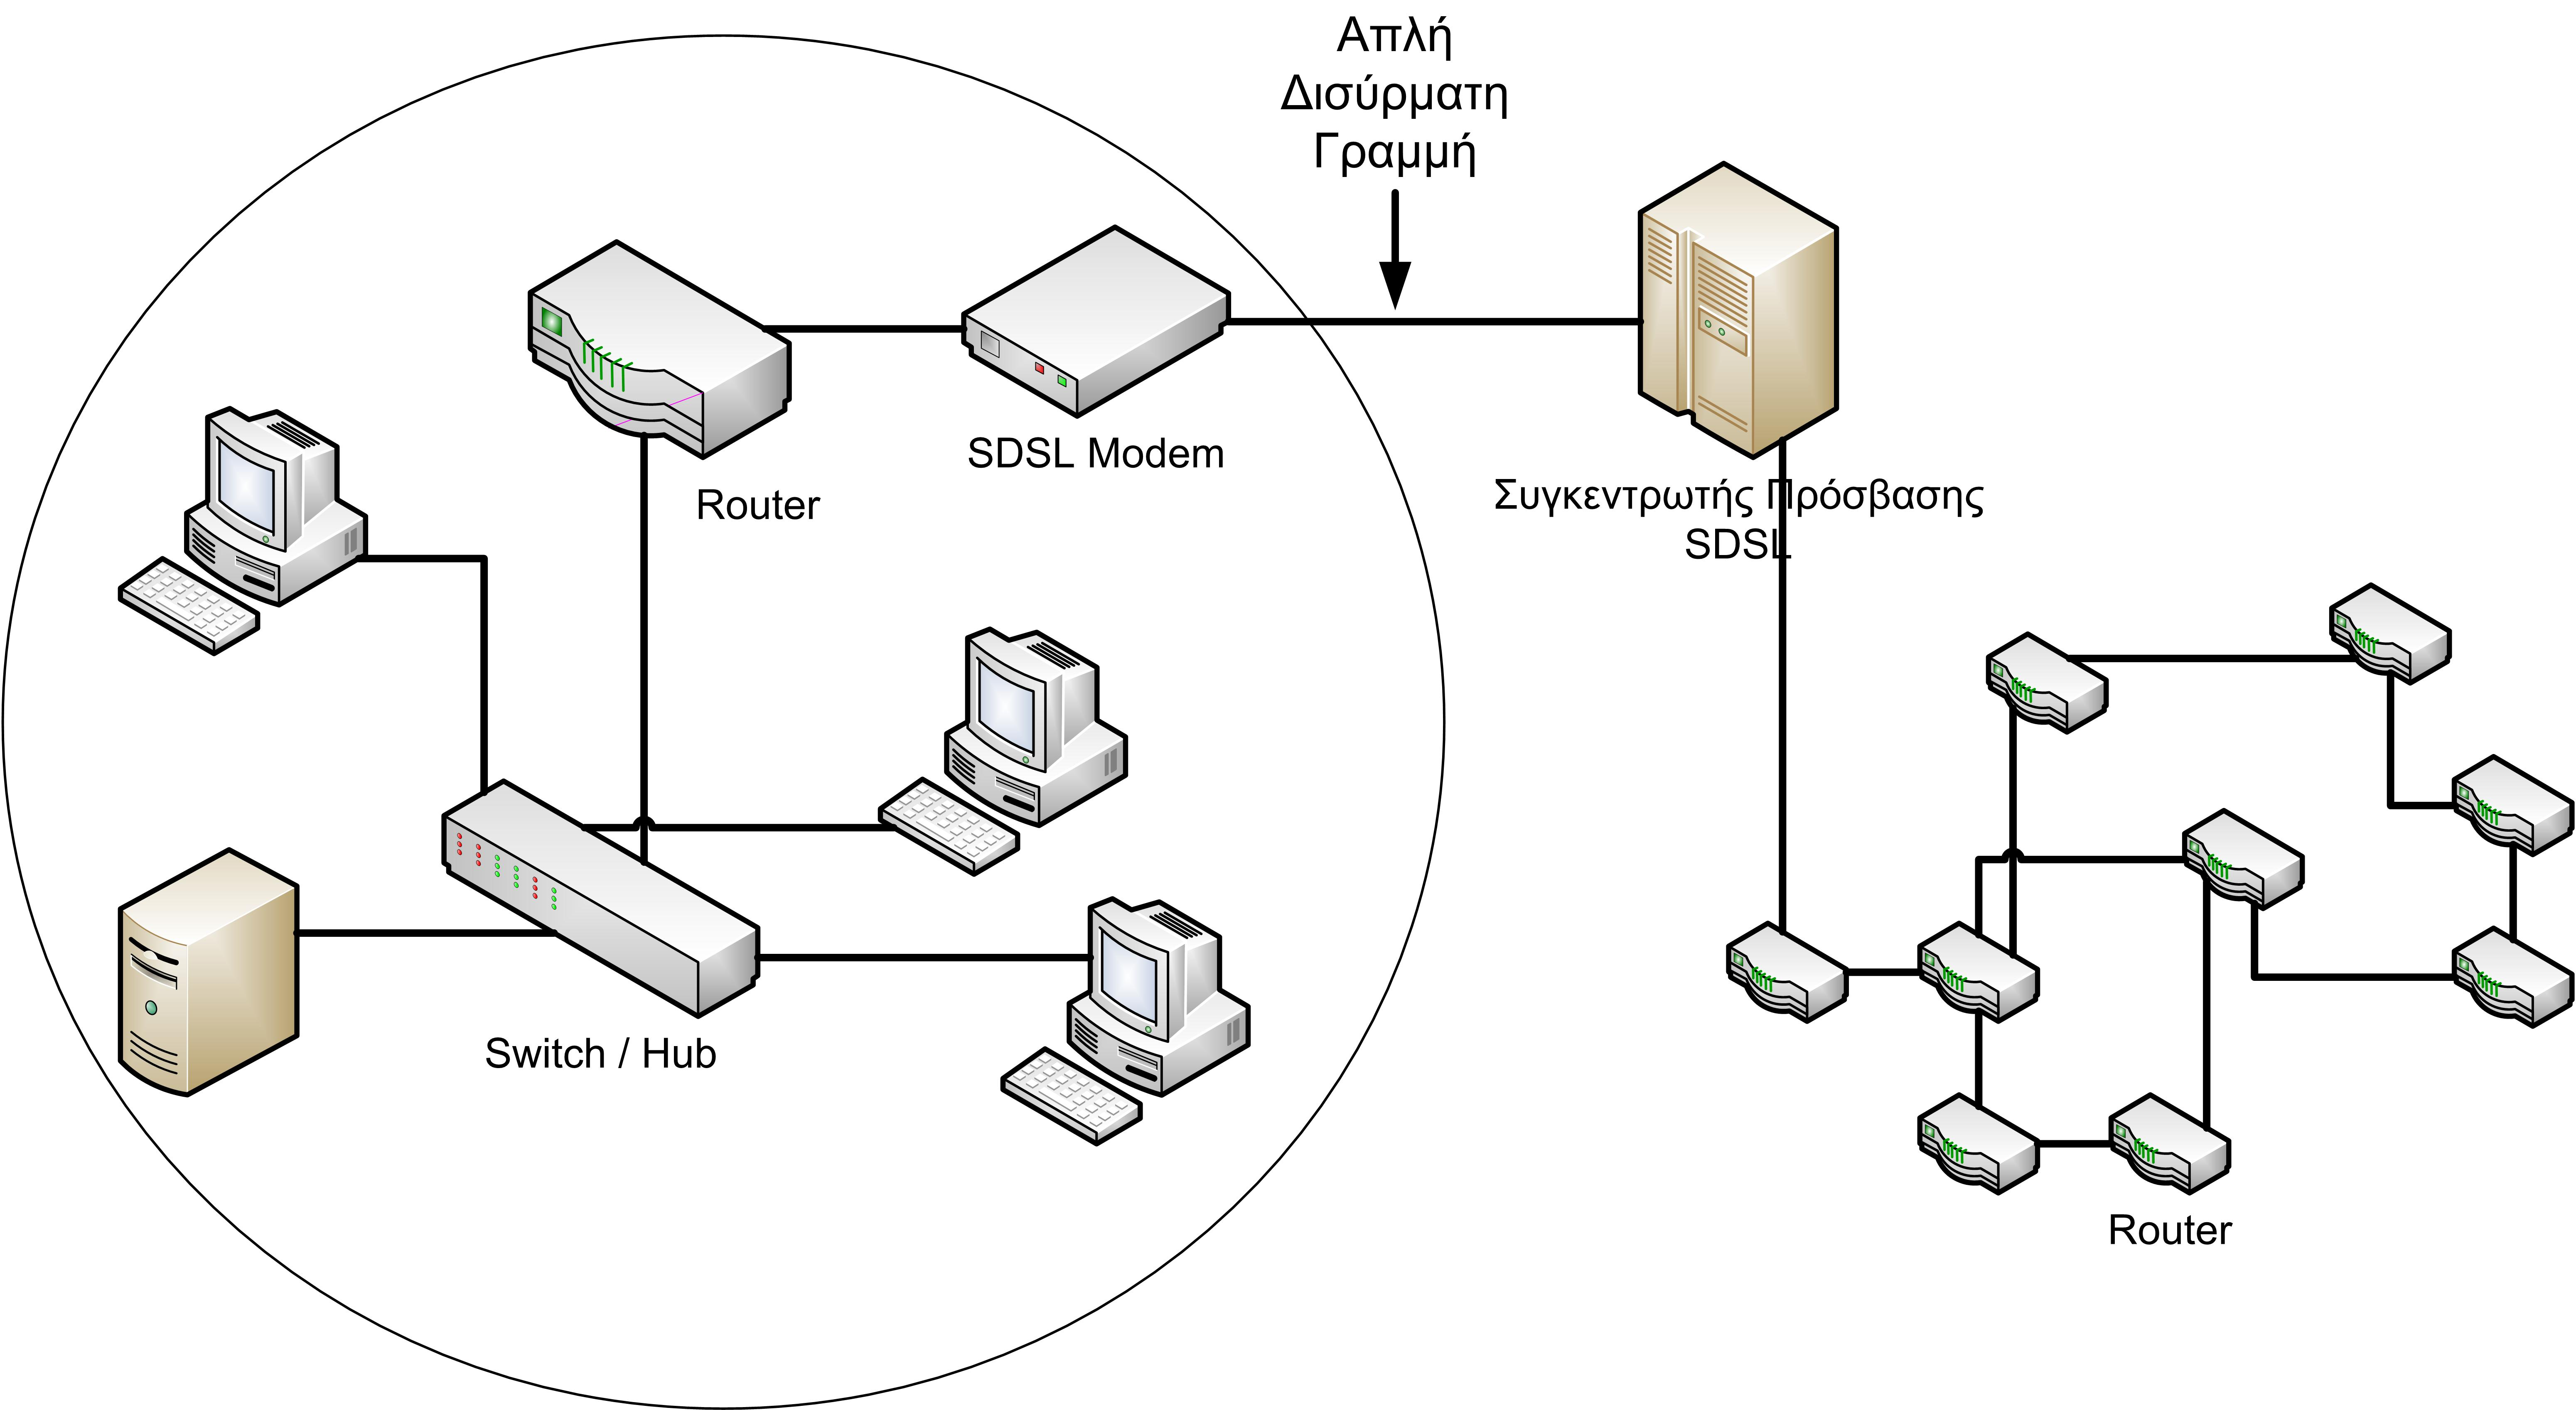
\includegraphics[width=0.95\textwidth]{images/chapter5/5-2}
  \caption {\textsl{Πρόσβαση Τοπικού Δικτύου σε Δίκτυο Ευρείας Περιοχής}}
  \label{5-2}
\end{figure}

Οι παραλλαγές xDSL υποστηρίζουν \emph{συμμετρική ή ασύμμετρη} μετάδοση δεδομένων. Στη συμμετρική μετάδοση η ταχύτητα είναι ίδια και προς τις δυο κατευθύνσεις (upstream και downstream) ενώ στην ασύμμετρη διαφορετικές (το upstream είναι μικρότερο).  Κάθε παραλλαγή είναι κατάλληλη για συγκεκριμένη χρήση:


\begin{itemize}
\item Η ασύμμετρη μετάδοση είναι κατάλληλη για χρήση όπου απαιτείται κατά βάση μεγαλύτερη ταχύτητα downstream, δηλαδή προς το χρήστη (π.χ. για πρόσβαση σε ιστοσελίδες και κατέβασμα αρχείων)
\item Η συμμετρική μετάδοση ενδείκνυται ως υποκατάστατο μισθωμένης γραμμής Ε1 και όπου απαιτείται υψηλή ταχύτητα μετάδοσης και προς τις δύο κατευθύνσεις (π.χ. για τηλεδιάσκεψη)
\end{itemize}
 
 Οι βασικές παραλλαγές xDSL είναι Α(symmetric)DSL, S(ymmetric)DSL, H(igh bit rate)DSL και V(ery high bit rate)DSL.
 
\begin{table}[!ht]
\begin{center}
\small
\begin{tabular}{|c|c|c|c|c|}
  \hline
    \multirow{2}{*}{}\textbf{Τεχνολογία}&\textbf{Σημασία}&\textbf{Αριθμός}&\textbf{Ταχύτητα}&\textbf{Μέγιστη} \\
    & & \textbf{Ζευγών} & & \textbf{Απόσταση} \\
  \hline
 \multirow{2}{*}{} ADSL & Asymmetric & 1 & 8 Mbps Downstream & 3 Km \\
    & DSL & & 1,5 Mbps upstream & 6,6 -- 7,5 Km\\
  \hline
 \multirow{2}{*}{} ADSL Lite & & 1 & 1 Mbps Downstream &  \\
    & & & 384 Kbps upstream & \\
  \hline
 \multirow{2}{*}{} HDSL & High-bit-rate & 2 & 2 Mbps full duplex (E1) & 3,5 -- 4,5 Km \\
    & DSL & 3 & 1,5 Mbps full duplex (T1) & \\
  \hline
 \multirow{2}{*}{} SDSL & Single-line DSL & 1 & 2 Mbps full duplex (E1) & 3 Km \\
    & & & 1,5 Mbps full duplex (T1) & \\
  \hline
 \multirow{2}{*}{} VDSL & Very-high-bit- & 1 & 13 -- 52 Mbps Downstream & 0,3 -- 1,4 Km \\
    & rate DSL & & 1,5 -- 12 Mbps upstream & \\
  \hline
\end{tabular}
\normalsize
\caption{\textsl{Τεχνολογίες x-DSL}}
\label{t5-1}
\end{center}
\end{table}
 
 Η ADSL (Asymmetric Digital Subscriber Line) παρέχεται στους περισσότερους οικιακούς χρήστες στην Ελλάδα. Η τεχνολογία προσφέρει μεγάλες ταχύτητες δεδομένων (κατάλληλη για φωνή, δεδομένα, κινούμενη εικόνα, γραφικά) και ταυτόχρονα μετάδοση φωνής. Ο ρυθμός λήψης (downstream) φτάνει μέχρι 8 Mbps και αποστολής (upstream) μέχρι 1 Mbps. Το εύρος ζώνης αυτό παρέχεται εξ'ολοκλήρου στο χρήστη (δεν το μοιράζεται με άλλους χρήστες) και η σύνδεση είναι συνέχεια ενεργή (always on), σε αντίθεση με τις παλιού τύπου συνδέσεις όπου γίνεται κλήση για τη σύνδεση και στο τέλος της επικοινωνίας γίνεται  αποσύνδεση. Η απόδοση της ADSL εξαρτάται σημαντικά από την απόσταση του χρήστη από τον τηλεπικοινωνιακό πάροχο (και από τη διατομή του καλωδίου που χρησιμοποιείται). Επιτυγχάνονται οι παρακάτω ταχύτητες:
 
 \begin{itemize}
 \item 1,5 ΜBps για απόσταση 5,5 Km
 \item 2,0 Mbps για απόσταση 4,9 Km
 \item 6,3 Mbps για απόσταση 3,6 Km
 \item 8.4 Mbps για απόσταση 2,7 Km
 \end{itemize}
 
Υπάρχουν επίσης οι πιο εξελιγμένες εκδόσεις ADSL, η \emph{ADSL2 και ADSL2+} που παρέχουν μεγαλύτερες ταχύτητες αξιοποιώντας με διαφορετικό τρόπο το εύρος ζώνης του καλωδίου. Η μέγιστη ταχύτητα στο ADSL2+ είναι τα 24 Mbps downstream και 1 Mbps upstream (ή σε περίπτωση που υλοποιεί το πρότυπο ITU G992.5 Annex M τα 24 ΜBps / 3,5 Mbps). Στην πράξη, σε αυτές τις ταχύτητες μπορούν να συνδεθούν πολλοί λίγοι χρήστες λόγω της απόστασης τους από το τηλεφωνικό κέντρο.
 
 \begin{table}[!ht]
\begin{center}
\small
\begin{tabular}{|c|c|c|c|c|}
  \hline
    \multirow{2}{*}{}\textbf{Όνομα} & \textbf{Κοινή} & \textbf{Μέγιστος Ρυθμός} & \textbf{Μέγιστος Ρυθμός} \\
    \textbf{Προτύπου} & \textbf{Ονομασία} & \textbf{Λήψης} & \textbf{Αποστολής} \\
  \hline
 \multirow{2}{*}{} ANSI T1.413-1998 & ADSL & 8 Mbit/s & 1 Mbit/s \\
    Issue 2 & & & \\
  \hline
  ITU G.992.1 & ADSL (G.DMT) & 8 Mbps & 1 Mbps \\
  \hline
  \multirow{2}{*}{}ITU G.992.1 & ADSL over POTS & 8 Mbps & 1 Mbps \\
   Annex A & & & \\
  \hline
  \multirow{2}{*}{}ITU G.992.1  & ADSL over ISDN & 8 Mbps & 1 Mbps \\
  Annex B & & & \\
  \hline
  ITU G.992.2 & ADSL Lite (G.Lite) & 1,5 Mbps & 0,5 Mbps \\
  \hline
  ITU G.992.3/4 & ADSL2 & 12 Mbps & 1 Mbps \\
  \hline
  \multirow{2}{*}{}ITU G.992.3/4 & ADSL2 & 12 Mbps & 3,5 Mbps \\
   Annex J & & & \\
  \hline
  \multirow{2}{*}{} ITU G.992.3/4  & RE-ADSL2 & 5 Mbit/s & 0,8 Mbit/s \\
  Annex L & & & \\
  \hline
  ITU G.992.5 & ADSL2+ & 24 Mbit/s & 1 Mbit/s \\
  \hline
  \multirow{2}{*}{}ITU G.992.5  & RE-ADSL2+ & 24 Mbit/s & 1 Mbit/s \\
  Annex L & & & \\
  \hline
  \multirow{2}{*}{}ITU G.992.5  & ADSL2+ & 24 Mbit/s & 3,5 Mbit/s \\
  Annex M & & & \\
  \hline
\end{tabular}
\normalsize
\caption{\textsl{Πρότυπα ADSL}}
\label{t5-2}
\end{center}
\end{table}
 
 Η υψηλή ταχύτητα της ADSL επιτυγχάνεται χάρη σε εξελιγμένους αλγορίθμους και ψηφιακή επεξεργασία σήματος (DSP, Digital Signal Processing) που συμπιέζουν σε μεγάλο βαθμό την πληροφορία που μεταδίδεται μέσα από τα τηλεφωνικά καλώδια καθώς και στη βελτίωση των μετασχηματιστών των αναλογικών φίλτρων και των μετατροπέων από αναλογικό σε ψηφιακό (ADC, Analog to Digital Converter).
 
 Στη μετάδοση φωνής της απλής τηλεφωνικής σύνδεσης χρησιμοποιείται μόνο η περιοχή συχνοτήτων από 0 Hz -- 4 KHz. Καθώς το καλώδιο μπορεί να μεταδώσει πολύ μεγαλύτερες συχνότητες, το επιπλέον εύρος ζώνης χρησιμοποιείται για τη μετάδοση δεδομένων.  Οι συνηθισμένοι οικιακοί χρήστες χρησιμοποιούν τη γραμμή περισσότερο για κατέβασμα παρά για ανέβασμα δεδομένων, έτσι το μεγαλύτερο εύρος ζώνης της γραμμής διατίθεται στο κανάλι downstream παρά στο upstream.
 
 Οι συχνότητες του καναλιού υποδιαιρούνται σε μικρότερες περιοχές των 4,3125 KHz που ονομάζονται bins. Τα modems τυπικά κατά την έναρξη της επικοινωνίας (training) ελέγχουν ξεχωριστά κάθε τέτοια περιοχή για να καθορίσουν ποιες από αυτές μπορούν να χρησιμοποιηθούν. 
 
 Η σύνδεση ADSL χρησιμοποιείται για τη μεταφορά δεδομένων από τον τελικό χρήστη μέχρι το τηλεφωνικό κέντρο της περιοχής. Στο τηλεφωνικό κέντρο διακλαδώνεται μέσω \href{https://el.wikipedia.org/wiki/Digital_subscriber_line_access_multiplexer}{DSLAM} και μεταβιβάζεται με γραμμές πολύ μεγαλύτερης ταχύτητας στον αντίστοιχο πάροχο υπηρεσιών Internet.
 
 \begin{figure}[!ht]
  \centering
  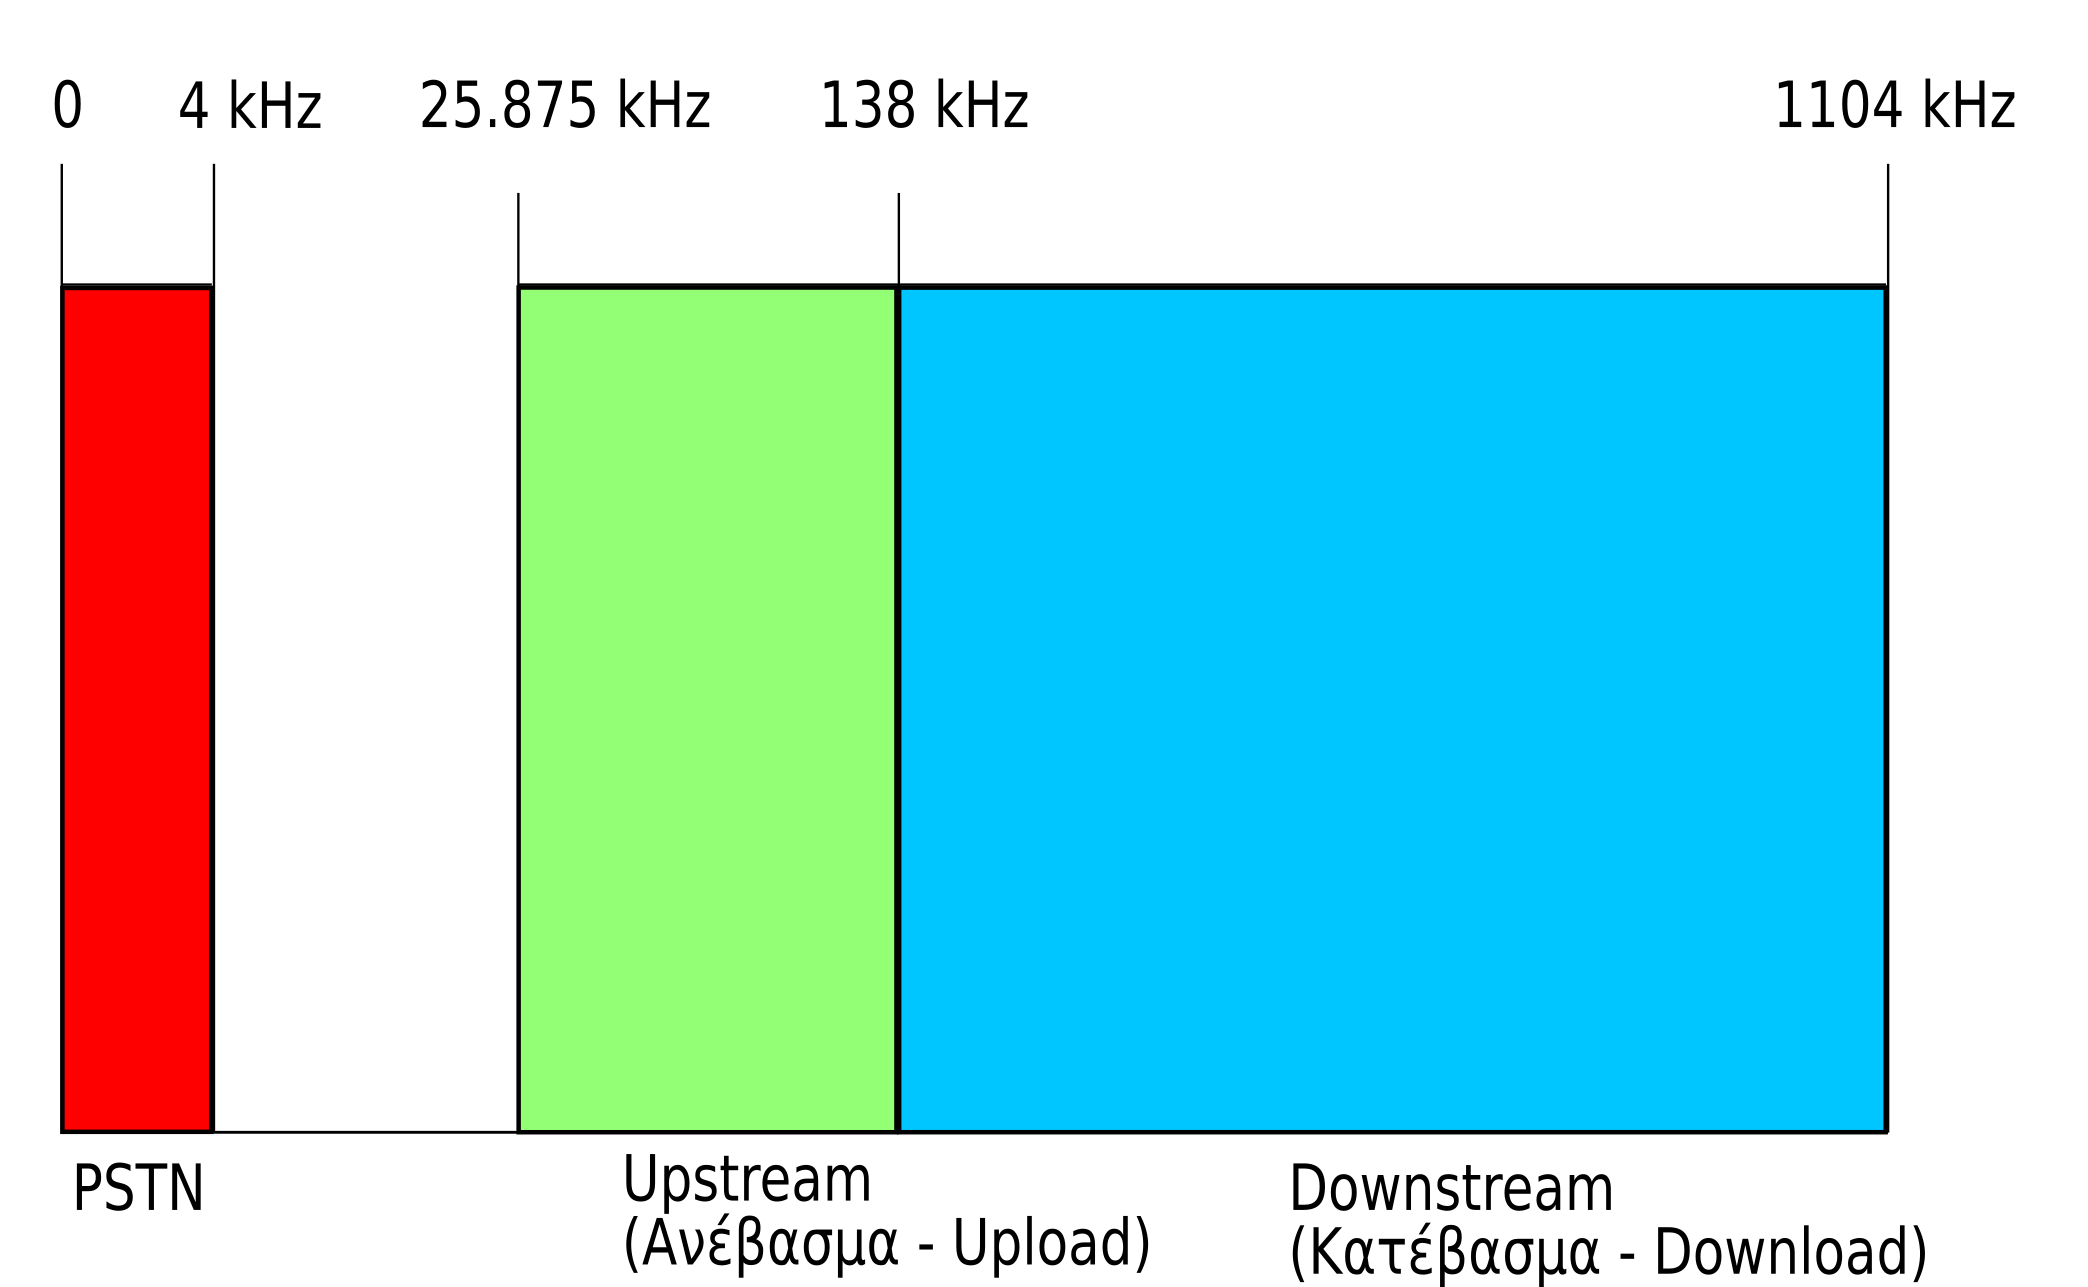
\includegraphics[width=0.95\textwidth]{images/chapter5/5-3}
  \caption {\textsl{Κατανομή Συχνοτήτων ADSL σε Γραμμή PSTN}}
  \label{5-3}
\end{figure}

Στο σχήμα \ref{5-3} φαίνονται οι περιοχές συχνοτήτων που χρησιμοποιούνται σε μια τηλεφωνική γραμμή PSTN που μεταφέρει δεδομένα ADSL. Με κόκκινο χρώμα φαίνεται η περιοχή συχνοτήτων φωνής (από 0 -- 4 KHz) με μπλε τα κανάλια για κατέβασμα (downstream) με και με πράσινο για ανέβασμα (upstream). 

Οι τηλεφωνικές γραμμές μεγάλου μήκους προξενούν μεγάλη εξασθένιση στα σήματα υψηλών συχνοτήτων. Στην συχνότητα του 1 MHz (που αντιστοιχεί στις συχνότητες Downstream ADSL/ADSL2+) η εξασθένιση μπορεί να φτάσει και τα 90 db.

\begin{inthebox}
\textbf{Πόσο μεγάλη εξασθένιση είναι τα 90 db;}

To decibel (db) δεν είναι από μόνο του μονάδα μέτρησης, αλλά χρησιμοποιείται για να συγκρίνουμε μεγέθη μεταξύ τους και λειτουργεί λογαριθμικά. Εξασθένιση 90 db σημαίνει ότι η ισχύς του σήματος μειώνεται κατά 10\textsuperscript{9} (1 δις!) φορές.\\
\end{inthebox}

Με τόσο μεγάλη εξασθένιση είναι προφανές ότι το κύκλωμα του ADSL modem εκτελεί αρκετά πολύπλοκες λειτουργίες προκειμένου να εξασφαλίσει το απαραίτητο εύρος ζώνης. Για να δημιουργηθούν πολλαπλά κανάλια επικοινωνίας τα ADSL modems χωρίζουν το διαθέσιμο εύρος ζώνης της γραμμής με ένα από τους δύο παρακάτω τρόπους:

\begin{itemize}
\item Πολυπλεξία με διαίρεση συχνότητας (Frequency Division Multiplexing)
\item Καταστολή της ηχούς (Echo Cancellation)
\end{itemize}

\begin{inthebox}
\textbf{Τι είναι η πολυπλεξία στη συχνότητα;}
Η πολυπλεξία στη συχνότητα είναι μια τεχνική που χρησιμοποιείται μαζί με τη διαμόρφωση για να περάσουμε περισσότερες από μια επικοινωνίες ταυτόχρονα μέσα από το ίδιο φυσικό μέσο, χωρίς να παρεμβάλλονται μεταξύ τους. Το πιο απλό παράδειγμα καθημερινής χρήσης που μπορούμε να δώσουμε είναι το ραδιόφωνο: έχουμε ένα μοναδικό κοινό φυσικό μέσο (τον αέρα) αλλά μπορούμε μέσα από αυτό να μεταδώσουμε πολλαπλά σήματα ίδιων ουσιαστικά συχνοτήτων (λόγος, μουσική, τραγούδι). Πως το επιτυγχάνουμε; Δεν μεταδίδουμε απευθείας τις συχνότητες της μουσικής στον αέρα, αλλά χρησιμοποιούμε διαμόρφωση για να ``φορτώσουμε'' το μουσικό σήμα σε μια άλλη υψηλότερη συχνότητα (αυτή στην οποία συντονίζουμε το ραδιόφωνο). Οι συχνότητες αυτές (φέρουσες) απέχουν αρκετά μεταξύ τους ώστε να μπορούμε να τις ξεχωρίσουμε με το κατάλληλο κύκλωμα και να ανακτήσουμε την αρχική πληροφορία (μουσική).

\textbf{Τι είναι η καταστολή της ηχούς;}
Όταν μεταδίδουμε ένα σήμα μέσα από μια γραμμή, δημιουργείται ηχώ. Καθώς το σήμα φτάνει στον αποδέκτη, ένα μέρος του ανακλάται στην άκρη της γραμμής και αρχίζει να επιστρέφει στον αποστολέα. Καθώς η ηχώ ταξιδεύει μέσα από την τηλεφωνική γραμμή παρεμβάλλει το κανονικό σήμα εξασθενώντας το. Αν πρόκειται για γραμμή που μεταφέρει μόνο ομιλία, η ηχώ προκαλεί χειροτέρευση της ποιότητας επικοινωνίας. Σε γραμμή που μεταφέρει και δεδομένα (όπως η DSL) η ηχώ μειώνει το διαθέσιμο εύρος ζώνης της γραμμής και προκαλεί επιπλέον εξασθένιση στο σήμα που μεταδίδεται. Για το σκοπό αυτό προσπαθούμε είτε να αποφύγουμε τη δημιουργία της, είτε να την καταστείλουμε αν έχει ήδη δημιουργηθεί. Στις γραμμές DSL αυτό γίνεται με ειδικά ηλεκτρονικά κυκλώματα καταστολής της ηχούς.\\
\end{inthebox}

\subsubsection*{Παραλλαγές xDSL}

\begin{itemize}
\item \textbf{HDSL:} High-bit-rate Digital Subscriber Line. Πρόκειται για συμμετρική παραλλαγή και προσφέρει τον ίδιο ρυθμό αποστολής και λήψης, μέχρι 2 Mbps. Η μέγιστη απόσταση των δύο άκρων δεν μπορεί να υπερβαίνει τα 3,5 km. Επίσης απαιτεί την εγκατάσταση δυο τηλεφωνικών γραμμών (δύο ζεύγη συνεστραμμένων καλωδίων). Νεότερες εκδόσεις είναι το HDSL2 (2 Mbps με ένα ζεύγος καλωδίων) και το HDSL4 (ίδια ταχύτητα με το HDSL2 αλλά με δύο ζεύγη καλωδίων για καλύτερη αξιοπιστία).
\item \textbf{SDSL:} To SDSL (Single-line Digital Subscriber Line γνωστό και ως Sym\-met\-ric Digital Subscriber Line) είναι τεχνολογία παρόμοια με το HDSL (συμμετρική) και με ίδιο ρυθμό μεταφοράς δεδομένων (μέχρι 2 Mbps) αλλά απαιτεί μόνο ένα συνεστραμμένο ζεύγος καλωδίων. Για αυτό το λόγο η μέγιστη απόσταση μεταξύ των δύο άκρων δεν μπορεί να ξεπερνά τα 3 Km.
\item \textbf{VDSL:} To VDSL (Very-high-data-rate Digital Subscriber Line) δίνει εντυπωσιακά μεγαλύτερες ταχύτητες που φτάνουν μέχρι τα 52 Mbps downstream και 12 Mbps upstream σε περιορισμένη όμως απόσταση μεταξύ των δύο άκρων. Ανάλογα με την υλοποίηση η απόσταση δεν μπορεί να ξεπερνά το 1,5 Km. Διάδοχος τεχνολογία είναι το VDSL2 με ταχύτητες πάνω από 200 Mbps σε πολύ μικρή απόσταση, 100 Mbps στα 500 μέτρα και 50 Mbps στο 1 χιλιόμετρο.
\end{itemize}

